\chapter{Mechanical Design}
\section{Introduction}
The robot meets the design specification shown in Table \ref{tab:roborodentia_reqs}. It consists of four subassemblies: the base platform, shooting mechanism, ball hopper, and control unit. Each section was first modeled in SolidWorks, an industry-standard solid modeling CAD program. The designed parts were then fabricated using a laser cutter or 3D printer and assembled with metric hardware. Figure \ref{fig:robot_photo} displays a photograph of the robot while figures \ref{fig:render_isometric} through \ref{fig:render_right} show standard view renders of the SolidWorks model. Note that the robot uses mecanum wheels (a type of omni-directional wheel) which are modeled here as regular wheels for simplicity.

\begin{table}[h]
	\centering	\caption{Roborodentia 2018 Mechanical Requirements}
	\begin{tabular}{cp{5in}}
		\hline 
		& Requirement \\ 
		\hline 
		1 & \ssp Maximum footprint of 12" x 14" or smaller at start of match but may expand up to 14" x 17" during match. \\ 
		\hline 
		2 & \ssp Maximum height of 14" at start of match but no restriction during match. \\ 
		\hline 
		3 & Robot may not disassemble into multiple parts. \\ 
		\hline 
		4 & Robot may not be airborne. \\ 
		\hline 
		5 & Shooting mechanisms may not accelerate balls past 50 feet per second. \\ 
		\hline 
	\end{tabular} 
	\label{tab:roborodentia_reqs}
\end{table}

\begin{figure}[H]   % [h] means here
	\centering \includegraphics[width=6in, height=7in, keepaspectratio]{figures/robot_photo.png}
	\caption{Photograph of Robot}	\label{fig:robot_photo}
\end{figure}
\begin{figure}[H]   % [h] means here
	\centering 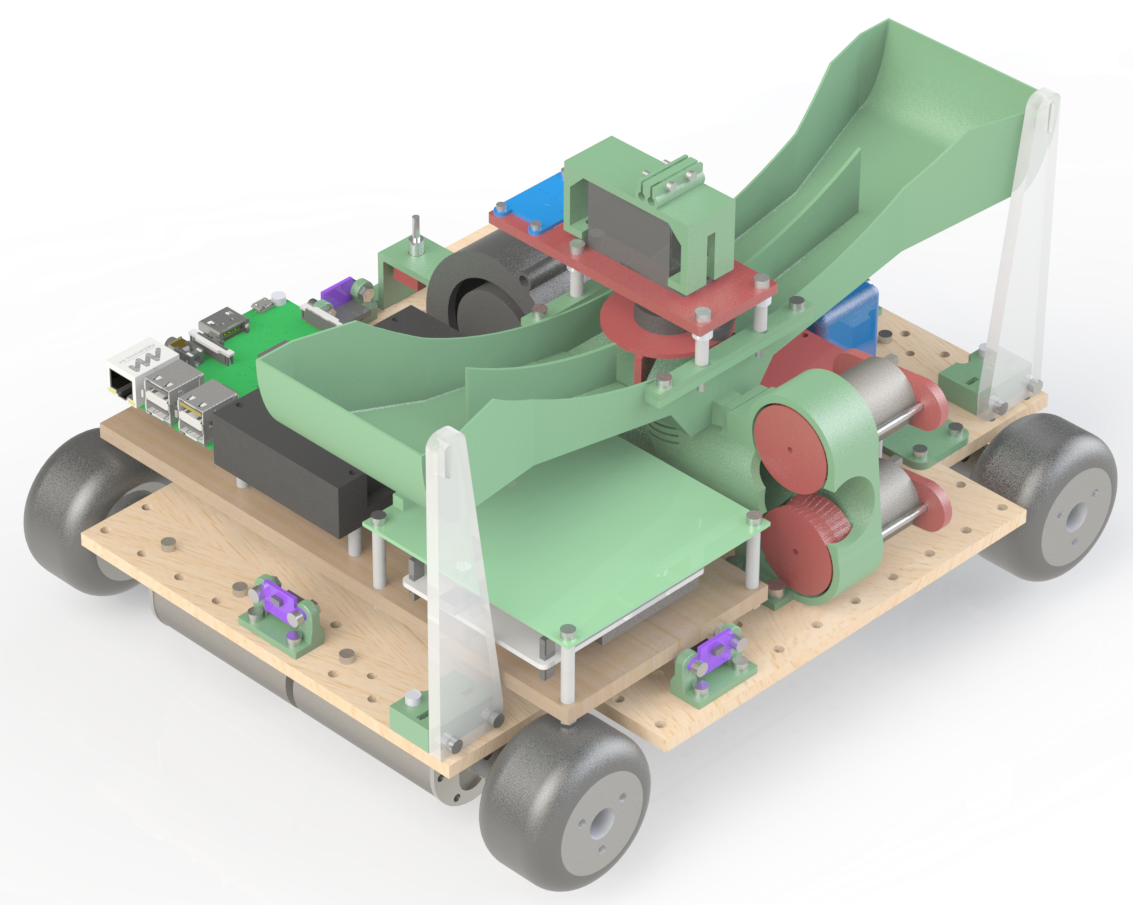
\includegraphics[width=6in, height=3.85in, keepaspectratio]{figures/render_isometric.png}
	\caption{Full Robot Render -- Isometric View}\label{fig:render_isometric}
\end{figure}
\begin{figure}[H]   % [h] means here
	\centering 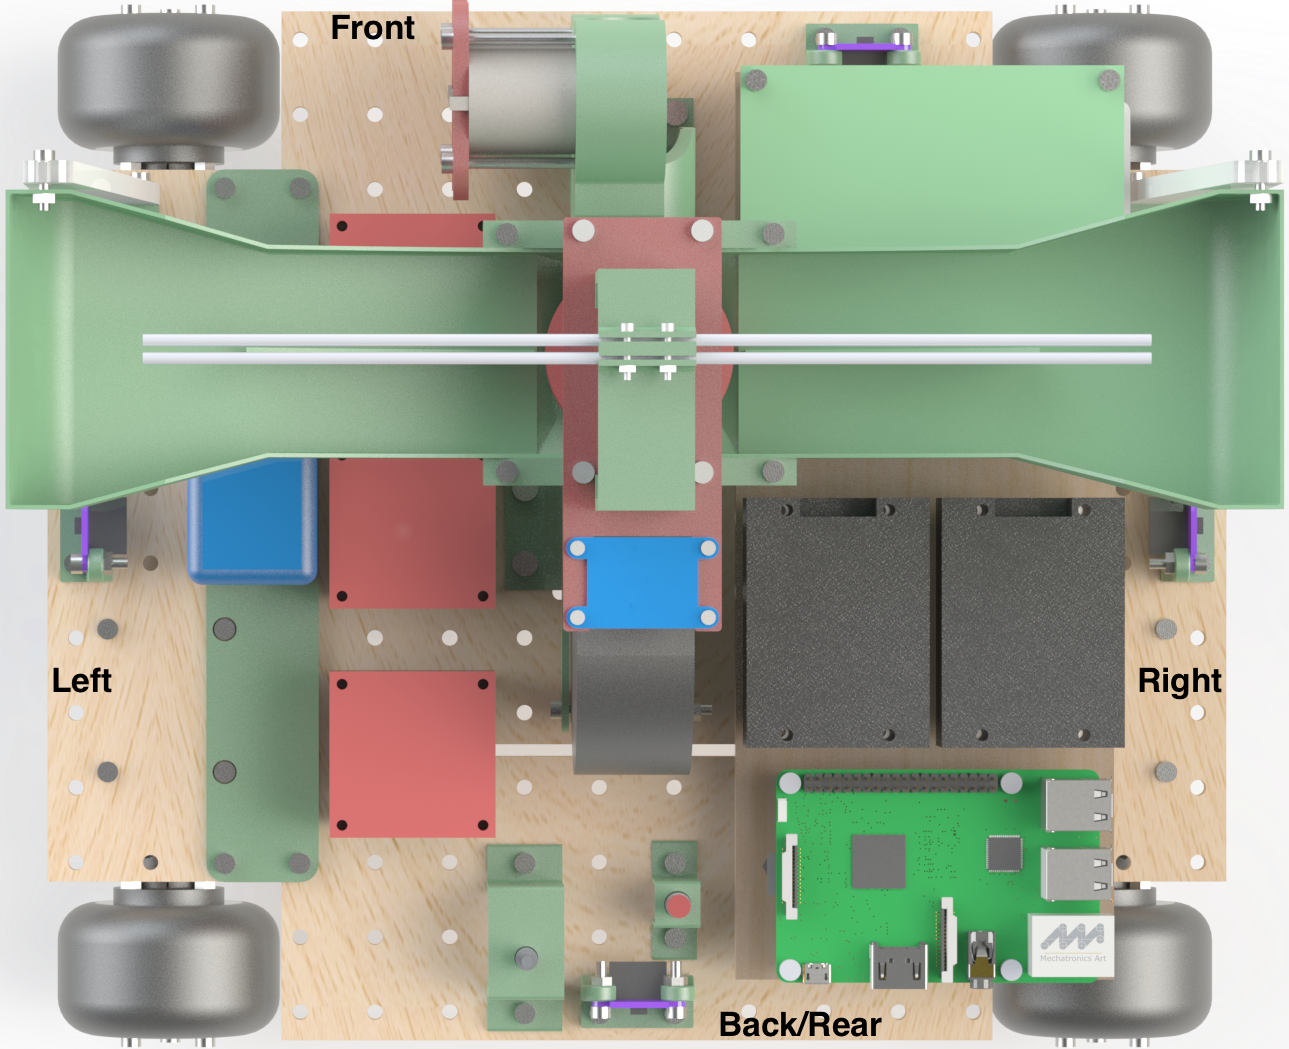
\includegraphics[width=6in, height=3.85in, keepaspectratio]{figures/render_top.png}
	\caption{Full Robot Render -- Top View}	\label{fig:render_top}
\end{figure}
\begin{figure}[H]   % [h] means here
	\centering 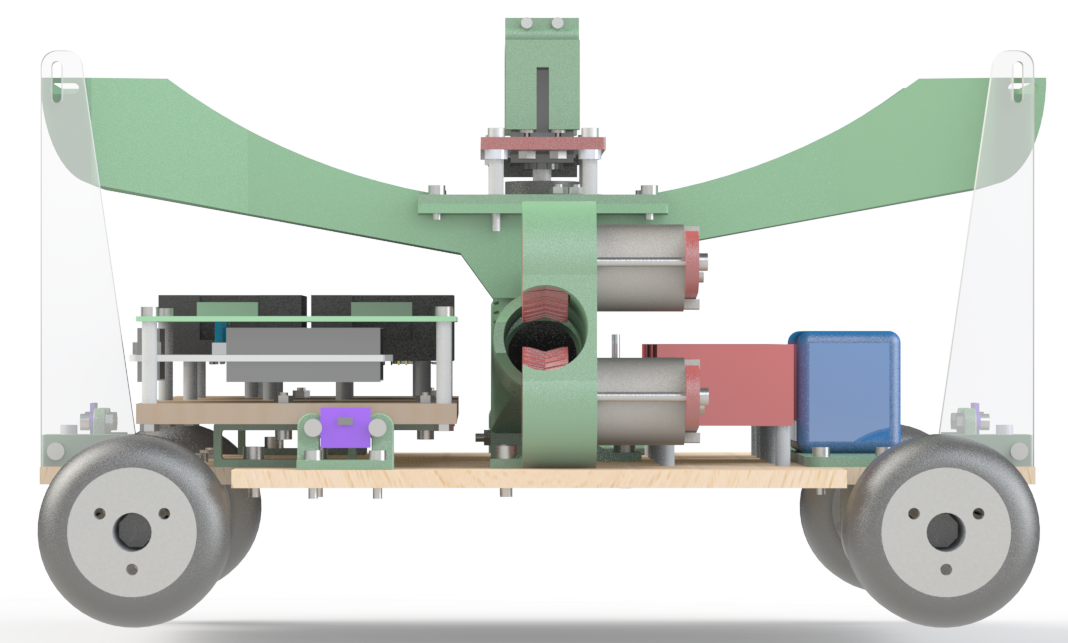
\includegraphics[width=6in, height=3.85in, keepaspectratio]{figures/render_front.png}
	\caption{Full Robot Render -- Front View}	\label{fig:render_front}
\end{figure}
\begin{figure}[H]   % [h] means here
	\centering 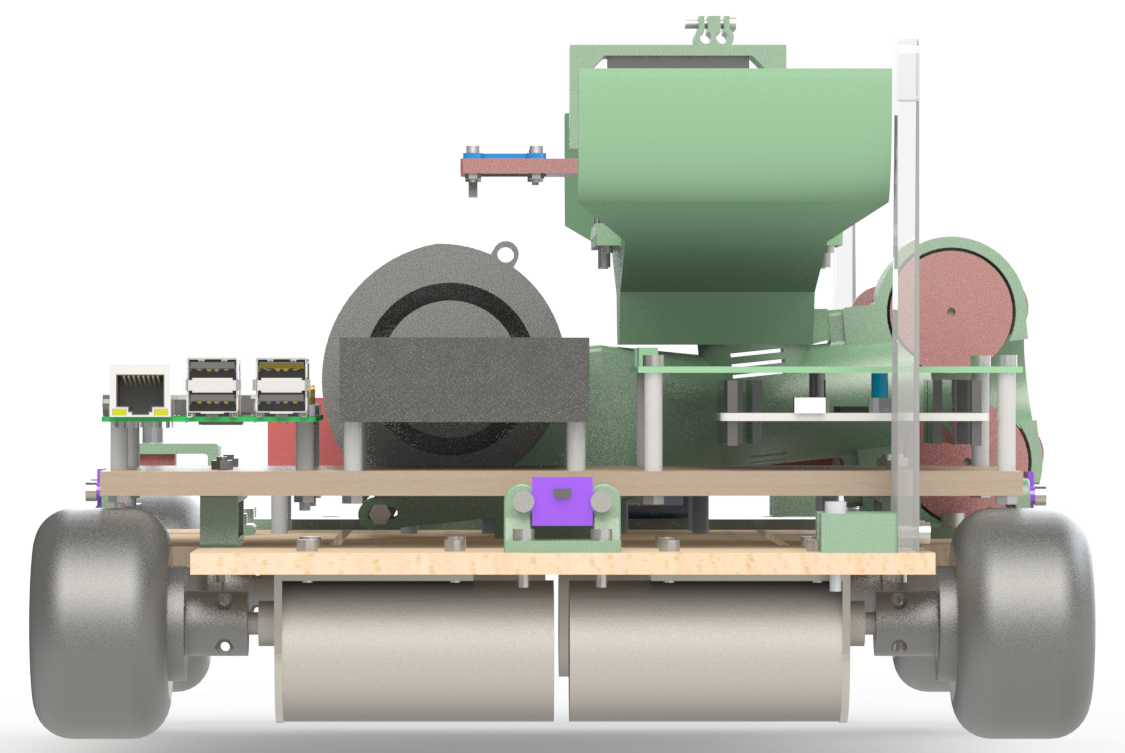
\includegraphics[width=6in, height=3.85in, keepaspectratio]{figures/render_right.png}
	\caption{Full Robot Render -- Right View}	\label{fig:render_right}
\end{figure}

\section{Base Platform}
The base platform of the robot, made from 1/4" medium density fiberboard (MDF), serves as the primary structural component and a mounting point for the motors, electronics, shooting mechanism, and hopper. The wood is laser cut with a 20 mm grid of 4.5 mm diameter holes to allow modular placement of components and the corner cutouts allow clearance for the wheels. Figures \ref{fig:base_platform} shows the assembled view of the subassembly.

\begin{figure}[H]   % [h] means here
	\centering 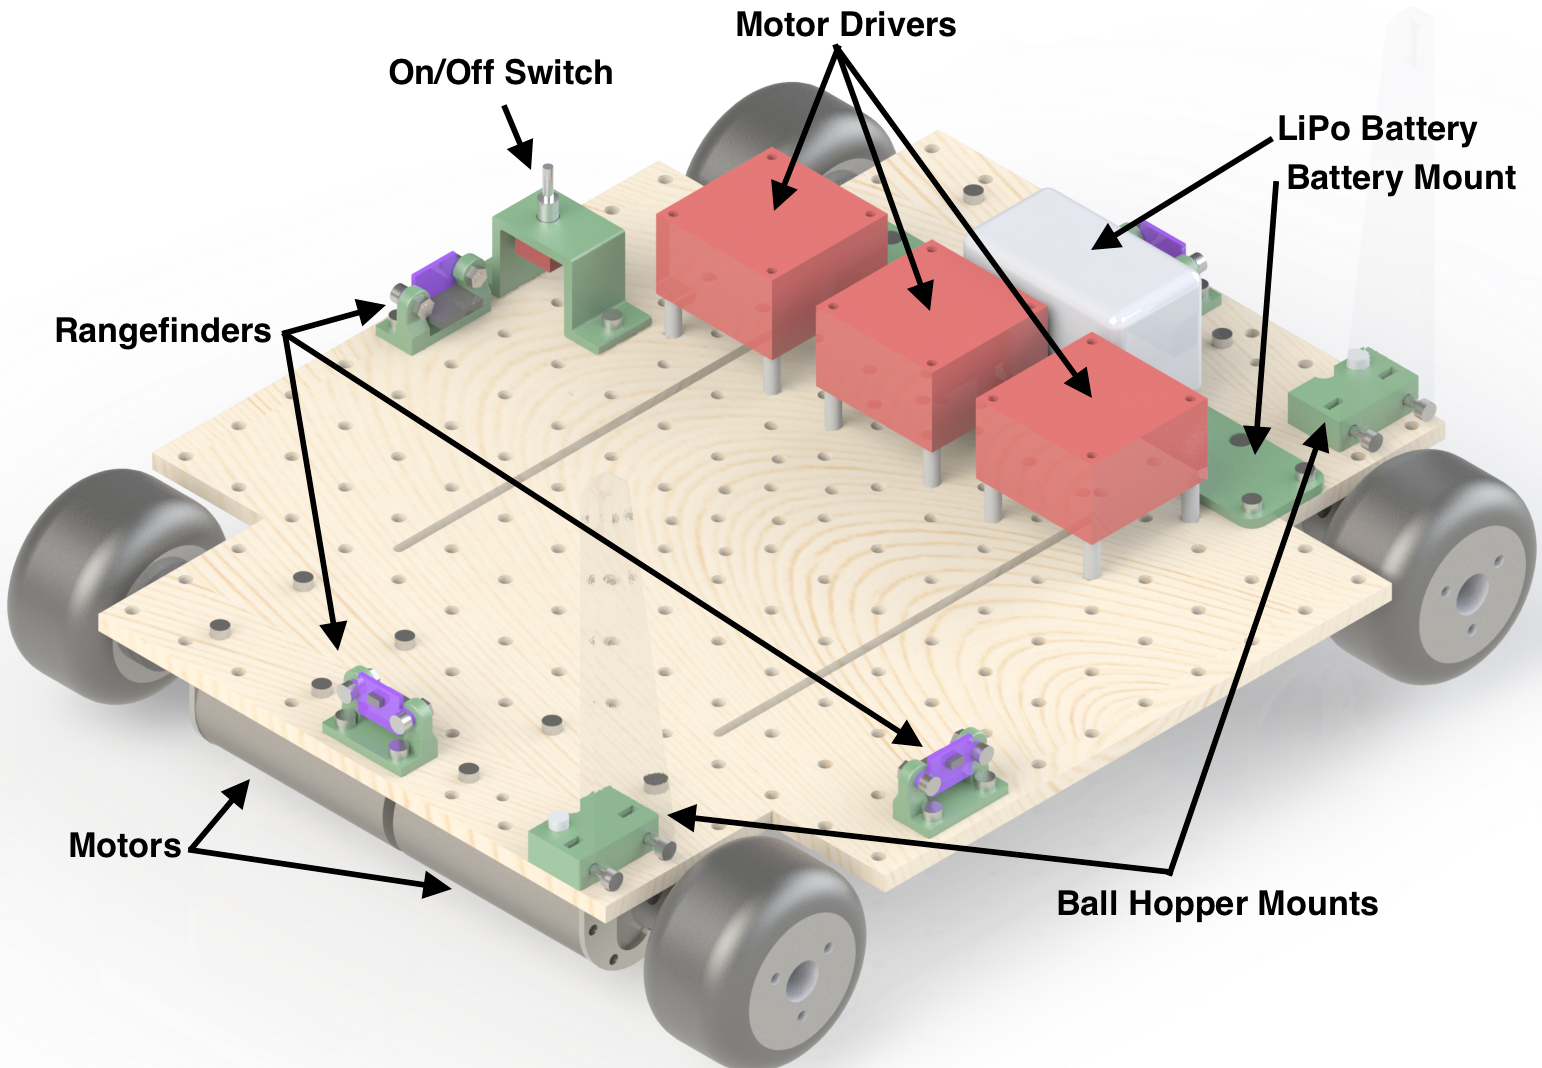
\includegraphics[width=6in, height=3.85in, keepaspectratio]{figures/base_platform.png}
	\caption{Base Platform}	\label{fig:base_platform}
\end{figure}

Four 12V Pololu 37D motors geared at a 70:1 ratio drive each of the 60 mm mecanum wheels. 3D printed couplings shown in Figure \ref{fig:wheel_coupler} connect the wheels to the D-shaped motor shafts. Each wheel contains eight angled rollers so unlike regular wheels which only produce a force vector perpendicular to the axis, mecanum wheels also produce a vector parallel to the axis. With the appropriate combination of speed and direction of each wheel, the robot can achieve simultaneous translation and rotation in any direction. 

\begin{figure}[H]   % [h] means here
	\centering 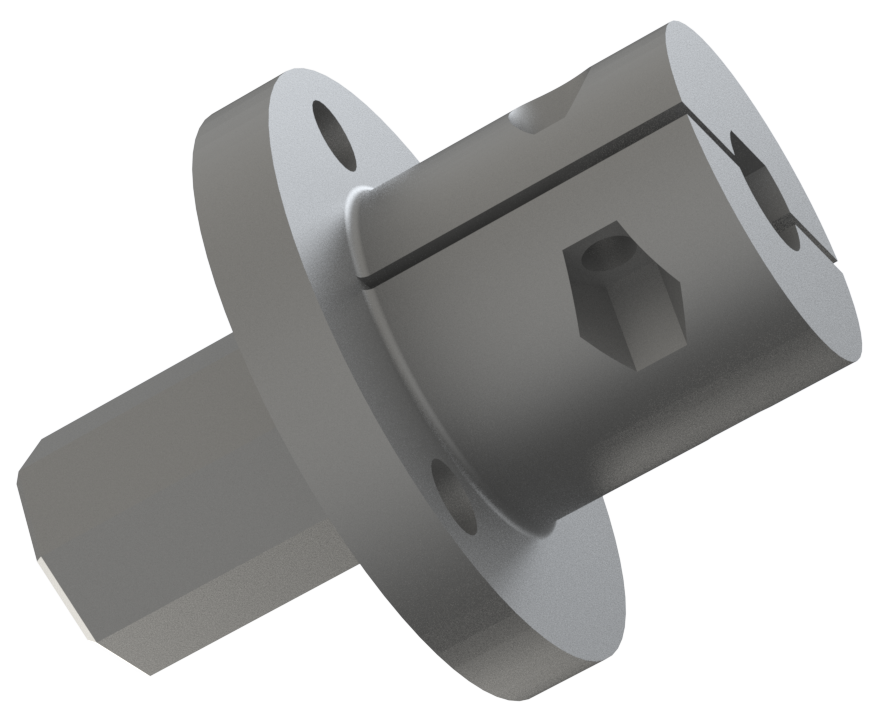
\includegraphics[width=6in, height=3.85in, keepaspectratio]{figures/wheel_coupler.png}
	\caption{Wheel Coupler}	\label{fig:wheel_coupler}
\end{figure}

Several electronic components are mounted directly on the base platform. Along the four edges of the platform, four ST Microelectronics VL53L0X laser rangefinders mounted on 3D printed brackets sense distance. These sensors cost between \$6 to \$20 mounted on a small PCB with supporting circuitry and can sense distances between 30 mm and 2000 mm at a rate of 30 Hz and less than 10\% error in most test conditions \cite{vl53l0x_datasheet}. A 4S, 1200 mAH LiPo battery powers the system through a on/off toggle switch. 

\section{Shooting Mechanism}
The shooting mechanism naturally takes inspiration from the official Nerf Rival Blaster toys since the manufacturer specifically optimized them to fire Nerf Rival balls in a way similar to baseball pitching machines. Figure \ref{fig:shooter_explode} shows an exploded view of the subassembly while Figure \ref{fig:shooter_top} displays the top view. The mechanism consists of two sections: the \textbf{barrel} (left green part in Figure \ref{fig:shooter_explode}) and the \textbf{wheel housing} (right green part in Figure \ref{fig:shooter_explode}). Both parts were fabricated using a fused deposition modeling (FDM) 3D printer as the geometries are highly complex. Therefore, the shooting mechanism consists of two separate components versus a unibody design to allow each half to be fabricated with optimal print direction, strength, and finish quality. The barrel is angled \ang{6} above horizontal, targeting the vertical center of the nets.

\begin{figure}[H]   % [h] means here
	\centering 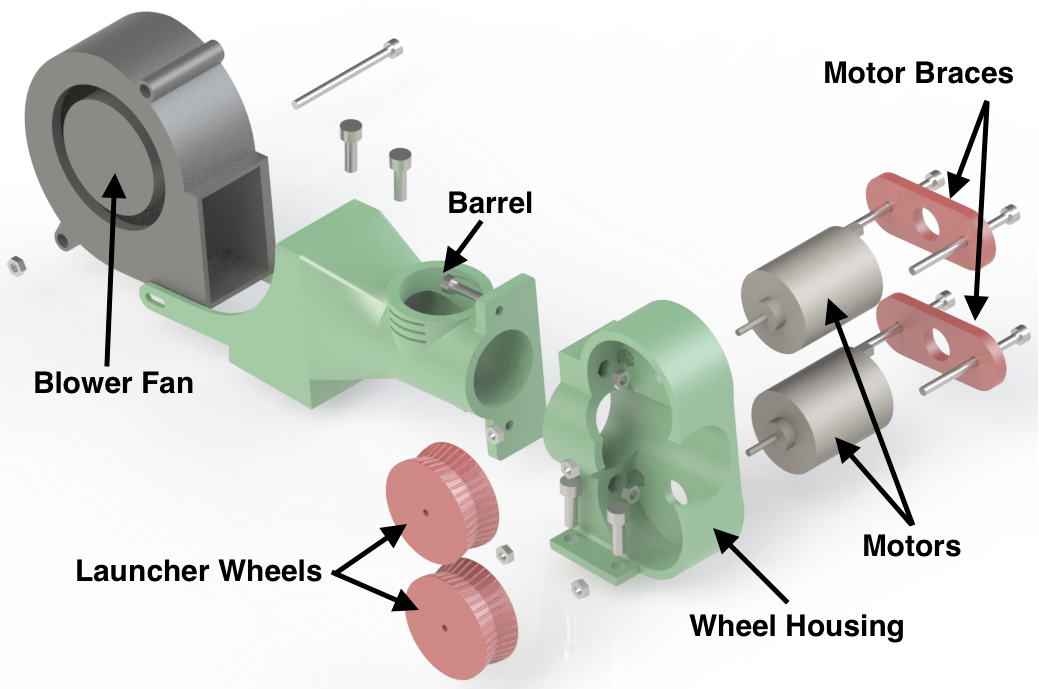
\includegraphics[width=6in, height=3.85in, keepaspectratio]{figures/shooter_explode.png}
	\caption{Shooting Mechanism -- Exploded View}	\label{fig:shooter_explode}
\end{figure}
\begin{figure}[H]   % [h] means here
	\centering 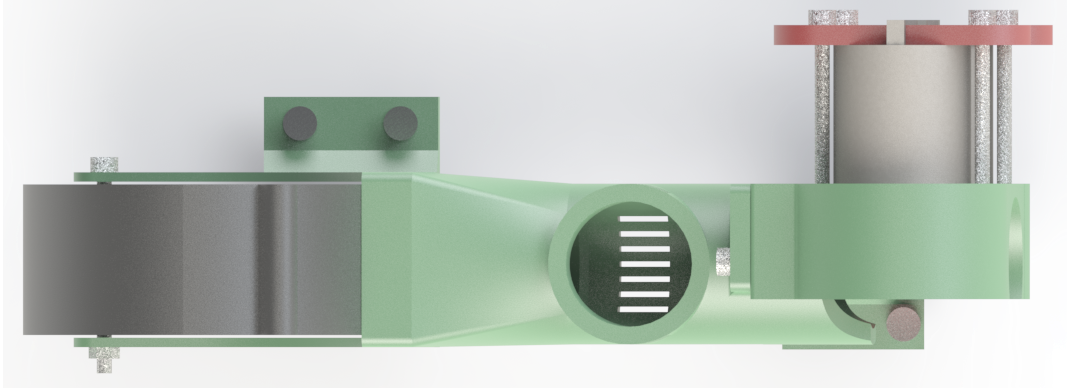
\includegraphics[width=6in, height=3.85in, keepaspectratio]{figures/shooter_top.png}
	\caption{Shooting Mechanism -- Top View}	\label{fig:shooter_top}
\end{figure}
\begin{figure}[H]   % [h] means here
	\centering 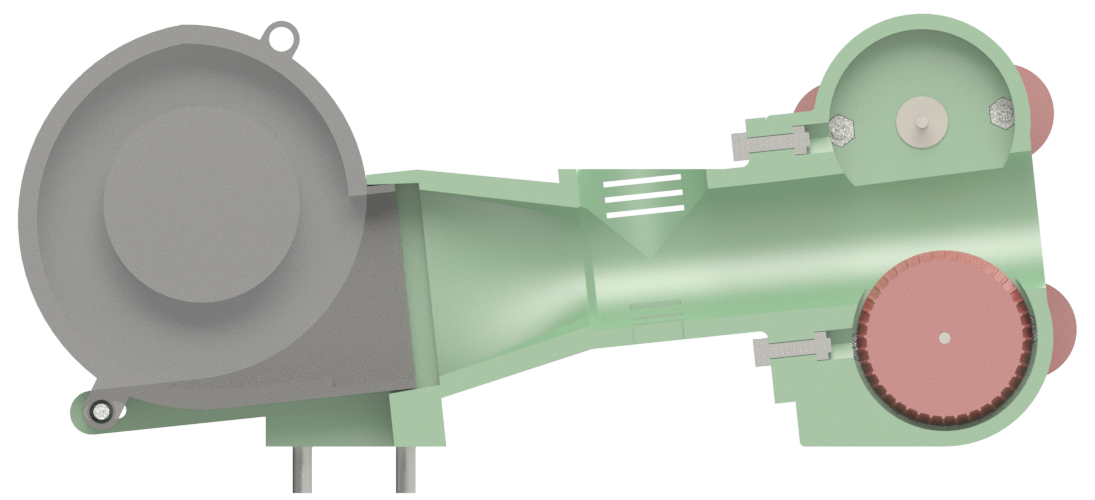
\includegraphics[width=6in, height=3.85in, keepaspectratio]{figures/shooter_xsec.png}
	\caption{Shooting Mechanism -- Cross Section View}	\label{fig:shooter_xsec}
\end{figure}

The \textbf{barrel} directs balls from the \textbf{ball hopper} to the \textbf{wheel housing}. First, the ball enters the barrel through a vertical chute by force of gravity. As the ball falls into the barrel, a high-pressure centrifugal (or blower fan) attached at the back of the barrel pushes it into the wheel housing inlet. As seen in Figure \ref{fig:shooter_xsec}, the barrel slightly narrows in the area behind the top chute to prevent the ball from rolling backwards towards the blower fan. A loft feature creates a smooth transition between the rectangular fan connection and the circular barrel. The foam balls, nominally 23 mm in diameter, would occasionally jam in a 24 mm barrel so all pathways are 25 mm. In the initial design, the pressure created by the blower fan was so high that it prevented the ball from falling down the vertical chute so strategically placed vents reduce the barrel pressure as the ball falls through the chute. As the ball travels down the chute into the barrel, it blocks the vents, increasing the pressure and forcing the ball into the wheel housing.

Inside the \textbf{wheel housing}, two counter-rotating 34mm wheels press fitted to two high-speed 12 V motors rapidly accelerate the foam ball up to 50 feet per second. The 14 mm gap between wheels compresses the ball to increase grip, thereby improving energy transfer. The motors lightly press fit into the wheel housing and are secured with 3D printed braces. The perimeter of each 3D printed wheel, detailed in Figure \ref{fig:shooter_wheel}, consists of a ribbed V-groove to increase the contact patch and grip with the compressed foam ball. Two "feet" with bolt holes at the bottom of the barrel and wheel housing secure the shooting mechanism to the base platform.

\begin{figure}[H]   % [h] means here
	\centering 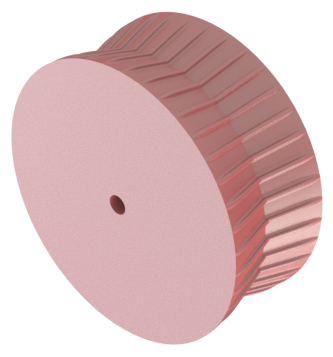
\includegraphics[width=6in, height=3.85in, keepaspectratio]{figures/shooter_wheel.png}
	\caption{Shooting Mechanism -- Shooter Wheel}	\label{fig:shooter_wheel}
\end{figure}

\section{Ball Hopper}
The robot must obtain the foam balls from supply tubes mounted on two sides of the side. The bottoms of the supply tubes are positioned seven inches above the floor and a swinging flap holds the balls in. The ball hopper, shown in Figure \ref{fig:ball_hopper} is a large 3D printed component designed to push the swinging flap away, collect the balls, store them, and dispense them into the shooting mechanism. Figure \ref{fig:ball_hopper_explode} shows an exploded view of the subassembly.

\begin{figure}[H]   % [h] means here
	\centering 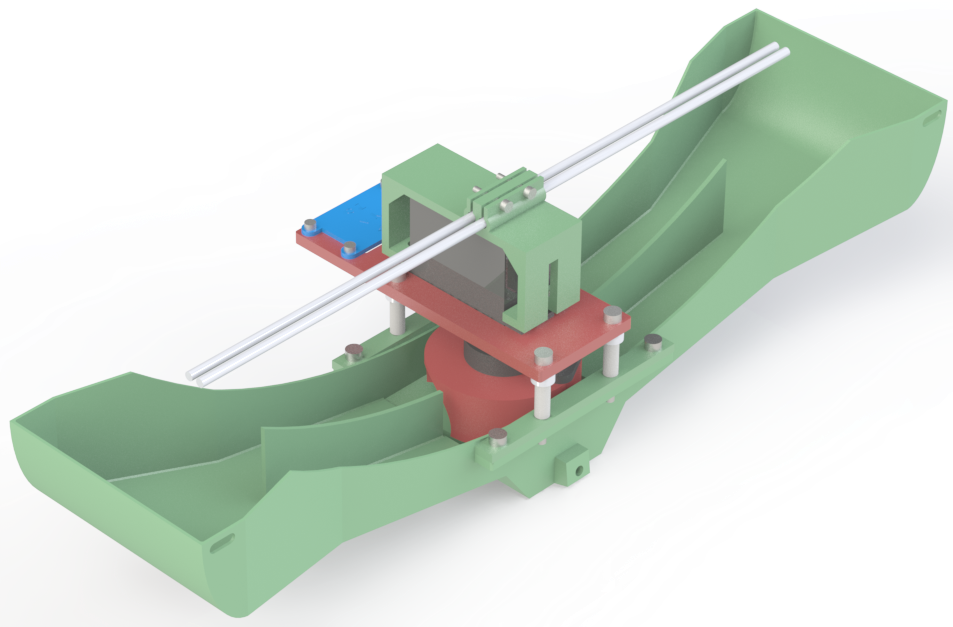
\includegraphics[width=6in, height=3.85in, keepaspectratio]{figures/ball_hopper.png}
	\caption{Ball Hopper}	\label{fig:ball_hopper}
\end{figure}

\begin{figure}[H]   % [h] means here
	\centering 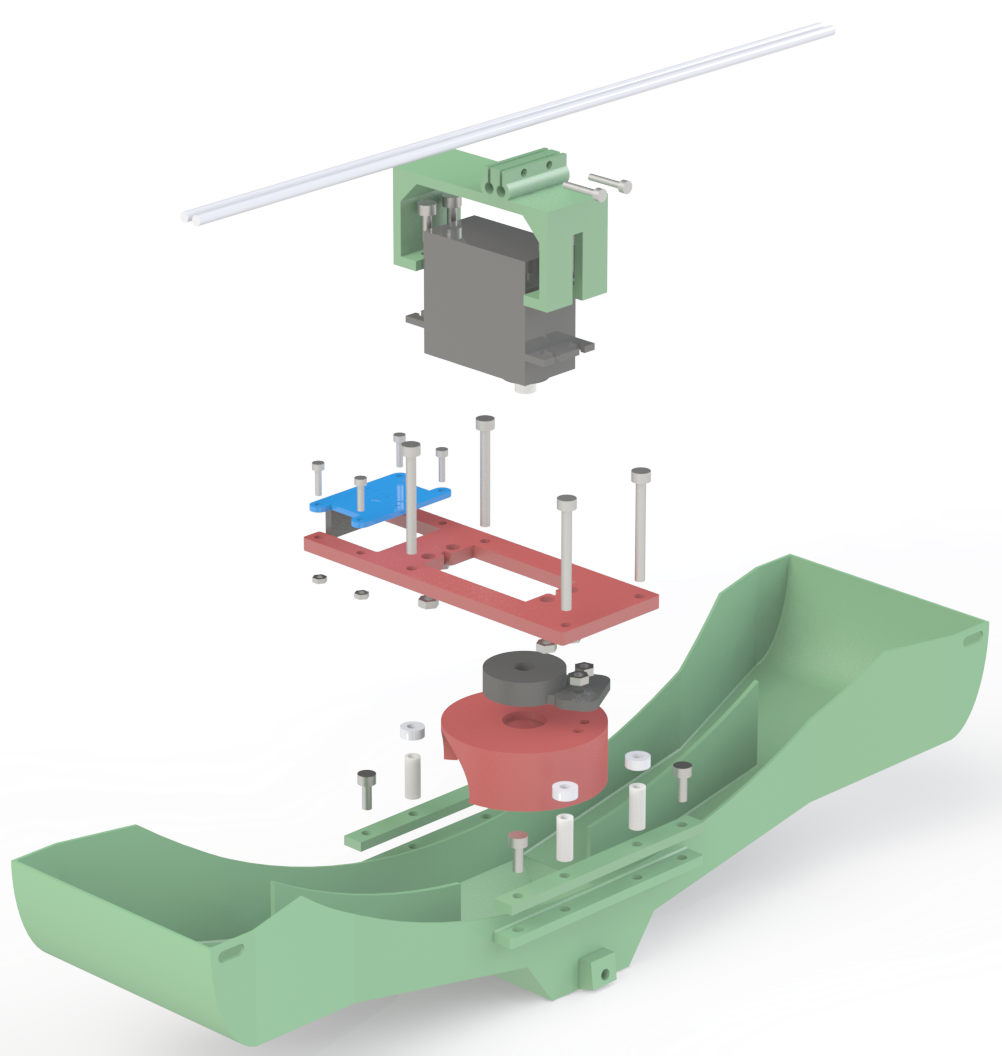
\includegraphics[width=6in, height=3.85in, keepaspectratio]{figures/ball_hopper_explode.png}
	\caption{Ball Hopper -- Exploded View}	\label{fig:ball_hopper_explode}
\end{figure}

First, the robot moves the hopper underneath the supply tube. As the flap swings open, the balls rolls down the steep sloped portion of the hopper. Visible in the cross section view of Figure \ref{fig:ball_hopper_xsec}, The slope rapidly becomes less steep in order to transition the balls downward momentum into sideways momentum, keeping balls from jamming against each other. The balls then roll into one of two channels before stopping at the dispensing gate.

\begin{figure}[H]   % [h] means here
	\centering 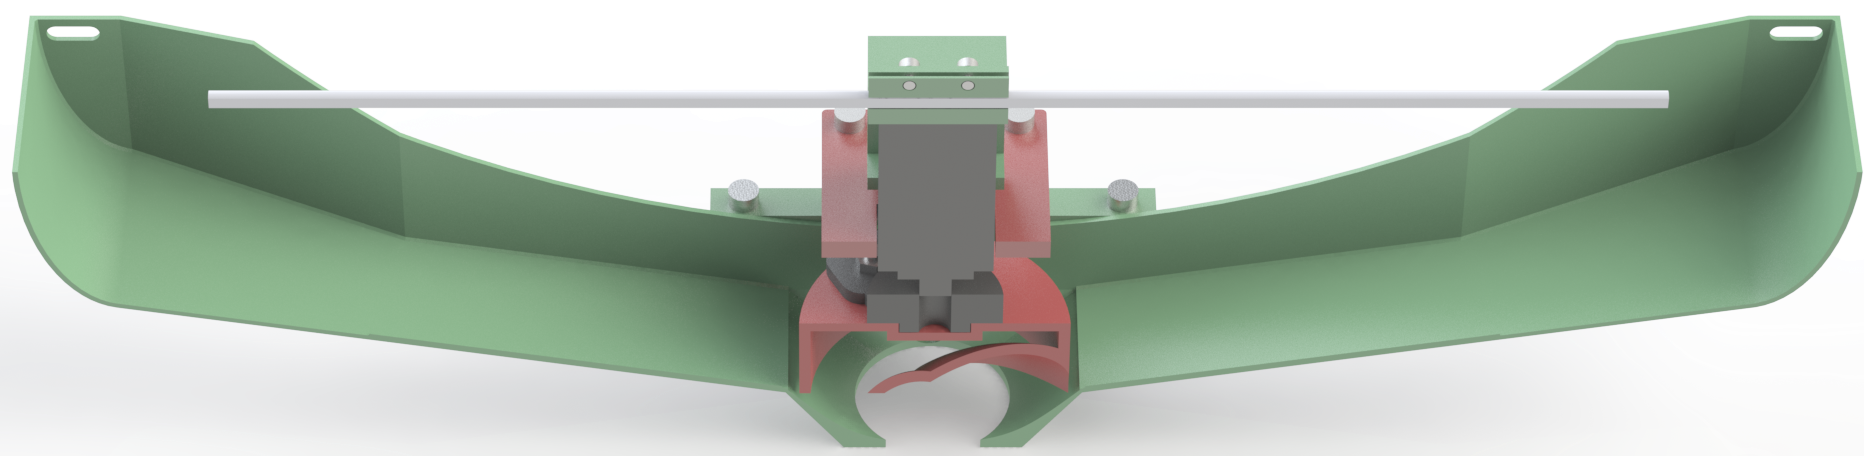
\includegraphics[width=6in, height=3.85in, keepaspectratio]{figures/ball_hopper_xsec.png}
	\caption{Ball Hopper -- Cross Section View}	\label{fig:ball_hopper_xsec}
\end{figure}

The dispensing gate, shown in Figure \ref{fig:dispensing_gate}, controls the movement of balls between hopper channel and shooting mechanism entrance. Its complex shape directs balls into the center of the ball hopper from one channel at a time to prevent jamming. A common \ang{180} movement servo, mounted in a 3D printed bracket above the center of the hopper, controls the dispensing gate. Fastened to the same bracket, an inertial measurement unit (IMU) measures magnetic compass heading and acceleration in three dimensions. 

\begin{figure}[H]   % [h] means here
	\centering 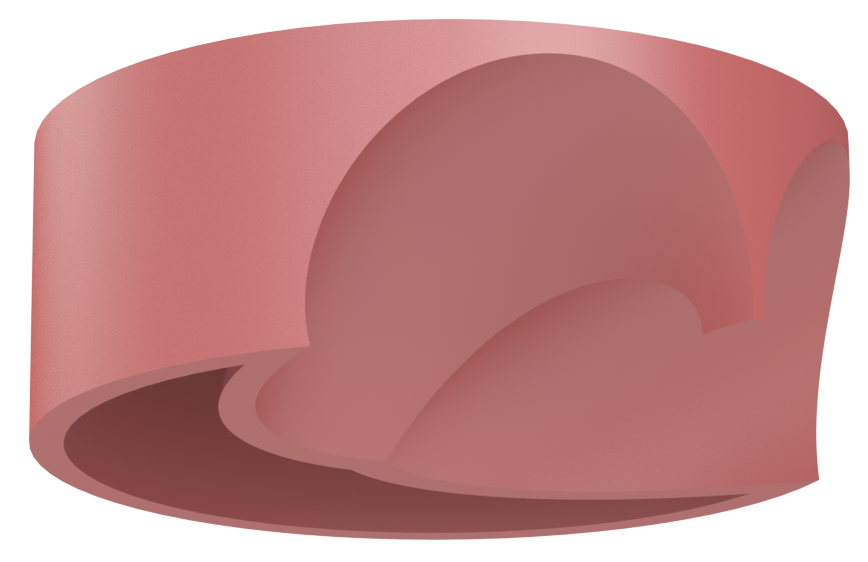
\includegraphics[width=4in, height=3.85in, keepaspectratio]{figures/dispensing_gate.png}
	\caption{Ball Hopper -- Dispensing Gate}	\label{fig:dispensing_gate}
\end{figure}

The ball hopper is mounted at three points: the top of the shooting mechanism and the left and right edges of the robot using 3D printed and acrylic braces shown in Figure \ref{fig:hopper_brace}. 

\begin{figure}[H]   % [h] means here
	\centering 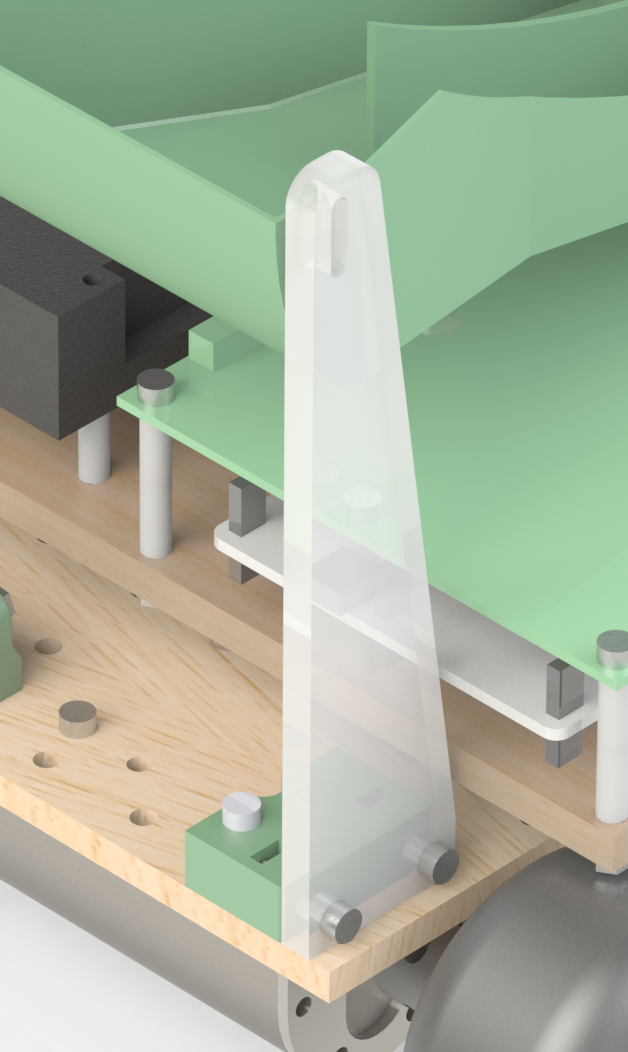
\includegraphics[width=6in, height=5in, keepaspectratio]{figures/hopper_brace.png}
	\caption{Ball Hopper -- Braces}	\label{fig:hopper_brace}
\end{figure}

\section{Control Unit}
The control unit, shown in Figure \ref{fig:control_unit}, consists of a 1/4" MDF board with various electronic components mounted: two off-the-shelf DC-DC switching converters, a custom interconnect printed circuit board (PCB), an off-the-shelf STM32 Nucleo-64 development board, and the Raspberry Pi computer. Two 3D printed standoffs, the green parts shown in Figure \ref{fig:control_unit_standoffs}, connect the control unit to the platform and raise it slightly to avoid colliding with the robot's wheels. 

\begin{figure}[H]   % [h] means here
	\centering 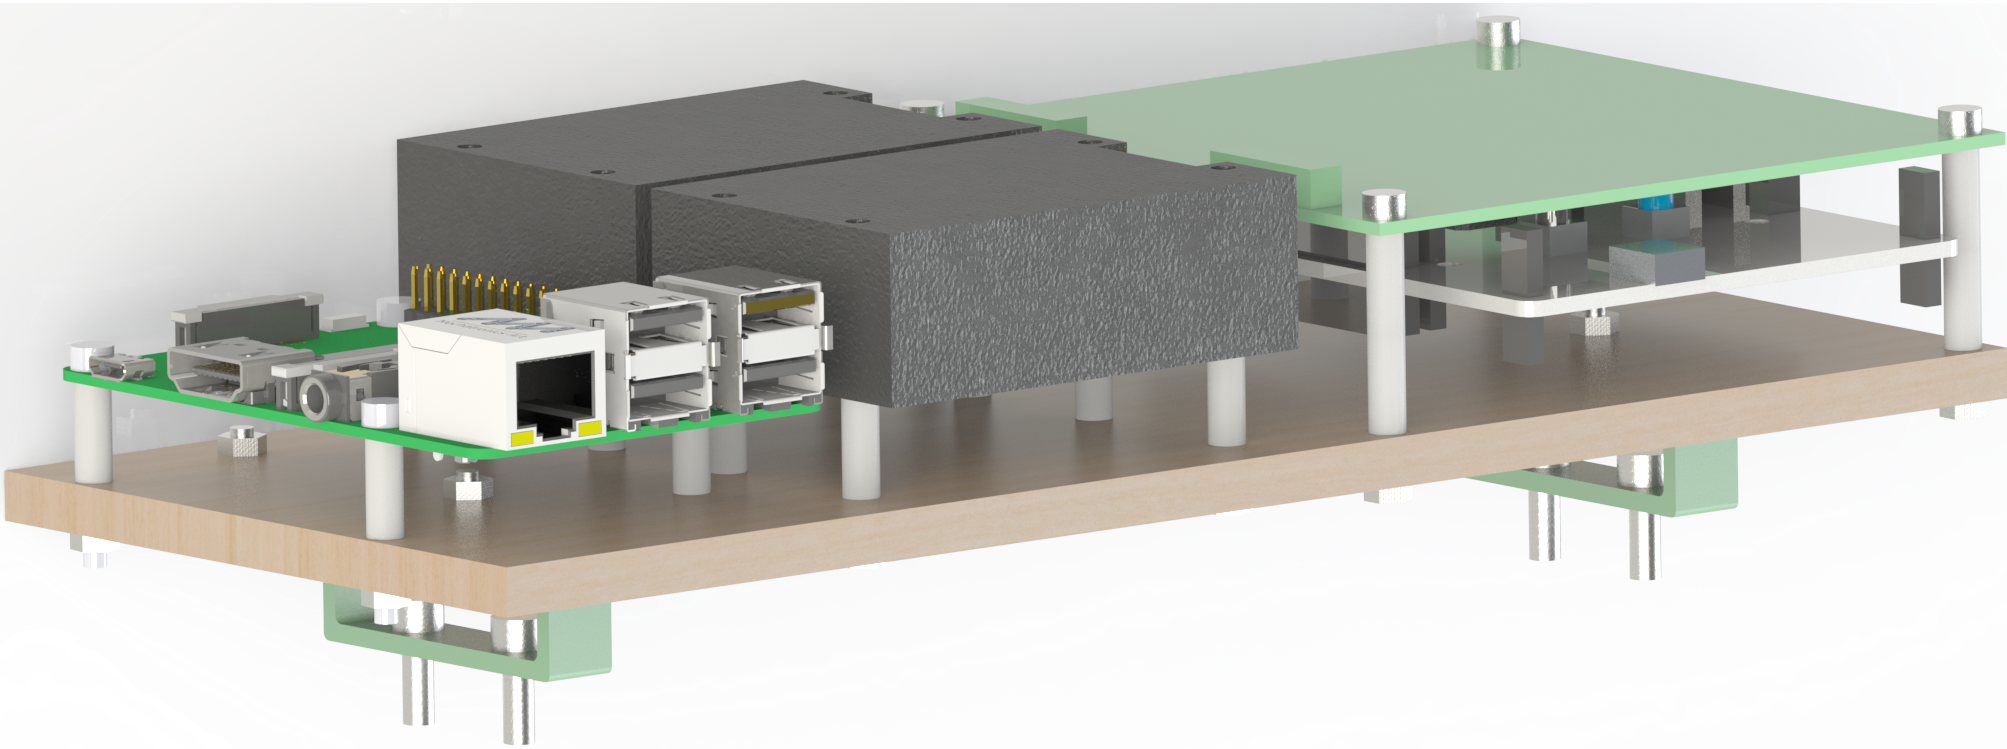
\includegraphics[width=6in, height=3.85in, keepaspectratio]{figures/control_unit.png}
	\caption{Control Unit}	\label{fig:control_unit}
\end{figure}

\begin{figure}[H]   % [h] means here
	\centering 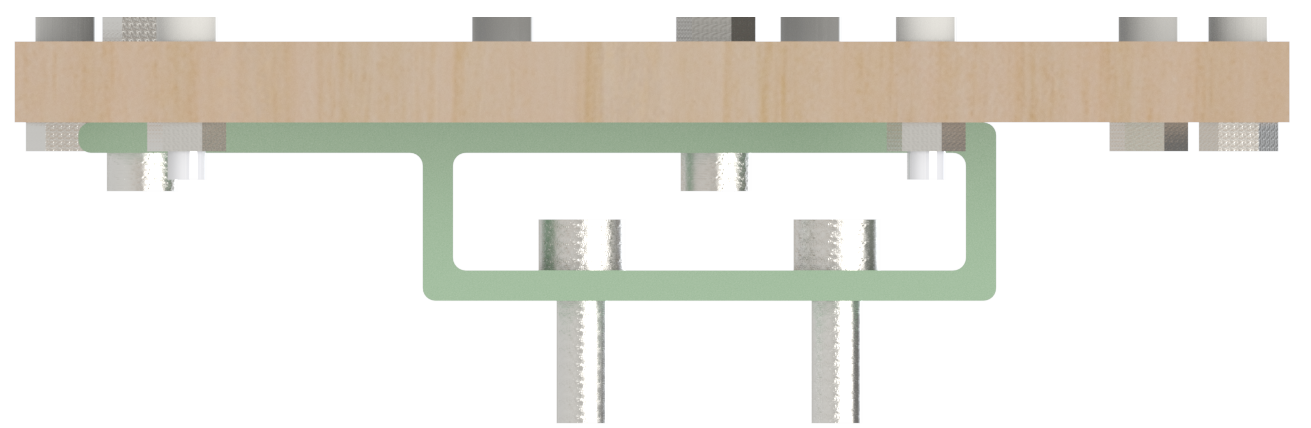
\includegraphics[width=6in, height=3.85in, keepaspectratio]{figures/control_unit_standoffs.png}
	\caption{Control Unit -- Standoffs}	\label{fig:control_unit_standoffs}
\end{figure}
